\section{Fazit}

\subsection{Heap oder List}

Die Holdback Queue mit internem Heap und mit interner Liste wurden in den obigen Plots in verschiedenen Szenarien getestet und verglichen. In Abbildung \ref{fig:auf_heapList} ist zu erkennen, dass bei aufsteigender Eingabeliste kein Unterschied zwischen den beiden Implementierungen zu erkennen ist. Wie in Kapitel \ref{Problemstellungen} beschrieben, werden die Elemente bei der Liste jeweils hinten angefügt, während hingegeben beim Heap alle Elemente an den nächsten leeren freien Index angefügt werden. Da beim Anfügen an die Liste durch die ganze Liste iteriert wird, beim Heap aber hingegen nur vom Wurzelelement aus das letzte freie Blatt gesucht werden muss, entsteht eine Komplexität von O(n) für die Liste und eine von O(log(n)) für den Heap. Beim Entfernen eines Elements hingegen, wird das erste Element der Liste abgeschnitten und mit dem Rest der Liste weitergearbeitet was eine Komplexität von O(1) zur Folge hat. Beim Heap hingegen muss das Wurzelelement entfernt und dann das neue Wurzelelement bestimmt werden was in O(2*log(n)) resultiert. Die Gesamtkomplexität ist also O(n) für die Liste und O(3*log(n)) für den Heap. Folglich sollte der Heap also schneller sein als die Liste.\\
Nun wurde im Benchmark allerdings immer die Delivery Queue mit eingebunden. Es lässt sich also schließen, dass diese so ineffizient ist, dass die Optimierungen der Holdback Queue wenig Einfluss auf den Gesamtprozess hat. Auch hier gilt 'Die Kette ist nur so stark wie das schwächste Glied', denn egal wie schnell ein Teilprozess Elemente verarbeitet, wenn der Nachfolgeprozess nicht mindestens genauso schnell ist, bildet sich im Nachfolgeprozess ein Stau und die Optimierung des ersten Teilprozesses wird hinfällig. Zur Bestätigung dieser Vermutung wurde eine Messung mit den einzelnen Holdback Queues durchgeführt (siehe Abbildung \ref{fig:real_hbqOnly}). Gemessen wurde hierbei nur der Prozess vom Eintritt der Nachrichten in die Holdback Queue, bis zum Verlassen mit aufsteigender und realer Eingabeliste.

\begin{figure}[htbp]
\begin{center}
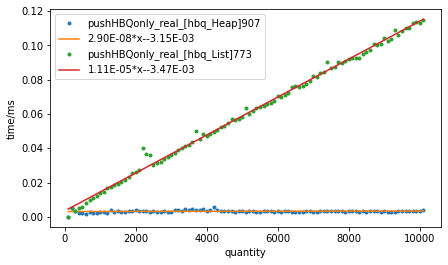
\includegraphics[scale=0.6]{Latex/Bilder/Plots/real_hbqOnly.png}
\caption{\label{fig:real_hbqOnly} real - vgl. List, Heap ohne Delivery Queue} 
\end{center}
\end{figure}

Hier ist der Unterschied zwischen den Implementierungen mit interner Liste und internem Heap klar zu erkennen. Die Trendlinien der aufsteigenden Eingabeliste sind nahezu identisch und die der real sortierten auch. Allerdings ist die Steigung der Holdback Queue mit interner Liste ca. 30° steiler. \\ Die Umsetzung der Holdback Queue mit einem internen Heap, um die Elemente besser zu sortieren, erweist sich also als durchaus effizient. Bei einer neuen Implementierung dieser gesamten Aufgabe sollte also auch die Delivery Queue und nicht nur die Holdback Queue optimiert werden. Eine mögliche Herangehensweise wäre es, die Sortierung der Delivery Queue zu verändern, sie also zum Beispiel absteigend zu sortieren. Dafür müsste analysiert werden, ob wirklich genauso viele Elemente in die Queue eingefügt, wie auch wieder gelöscht werden, wie es in Kapitel \ref{dlq} angenommen wurde. Ein Ausgang dieser Analyse könnte sein, dass nach Terminierung der Holdback Queue keine weiteren Elemente mehr in die Delivery Queue eingefügt werden müssen und somit auch keine mehr aus dieser gelöscht werden. Somit wäre also eine Delivery Queue mit absteigender Liste effizienter, da das von Erlang angebotene 'aneinander-pipen' von Elementen schneller ist, als der '++' Operator.

% Anhang mit entwürfen
\subsection{Limit der Delivery Queue}

Die Plots aus Abbildung \ref{fig:real_heapListPercent} und Abbildung \ref{fig:rand_heapListPercent} zeigen, wie groß der Einfluss des Delivery Queue Limits auf die Gesamtlaufzeit ist. Je kleiner dieses Limit hier ist, desto schneller ist der Prozess. Da die Elemente ab erreichen einer Holdback Queue Größe von 2/3 des Delivery Queue Limits von der Holdback an die Delivery Queue weitergegeben werden, wird bei einem kleineren Delivery Queue Limit mit kleineren Holdback Queues gearbeitet. Ein Element in eine kleinere Liste oder einen kleineren Heap einzufügen dauert dementsprechend weniger, da weniger Iterationen durchgeführt, bzw. Teilbäume gesucht werden müssen

\subsection{Pattern Matching}
Pattern Matching um die Effizienz der Holdback Queue zu erhöhen, hat sich anhand der Plots aus Abbildung \ref{fig:auf_hbq_pattern} und Abbildung \ref{fig:real_hbqAll}, im Widerspruch zur Annahme aus Kapitel \ref{erwartungen} eher als wenig maßgebend erwiesen. 

Da vorherige Auswertungen der Plots bereits erwiesen haben, dass die Delivery Queue einen starken Einfluss auf die Laufzeiten haben, wurde eine weitere Messung durchgeführt (siehe Abbildung \ref{fig:auf_hbqOnly_pattern}). In dieser wird mit einer Eingabeliste, welche bis zu 25000 Elementen in aufsteigend sortierter Reihenfolge hat, noch einmal die Holdback Queue mit und ohne Pattern Matching gemessen. Die Queue ohne Pattern Matching ist anfangs noch leicht ineffizienter, dessen Trendlinie verläuft aber leicht flacher als die der Holdback Queue mit Pattern Matching. Da die Zeiten der Messdurchläufe hier sehr gering sind ist die Streuung sehr hoch. Da diese aber sehr willkürlich ist, wird sie nicht weiter ausgewertet.

\begin{figure}[htbp]
\begin{center}
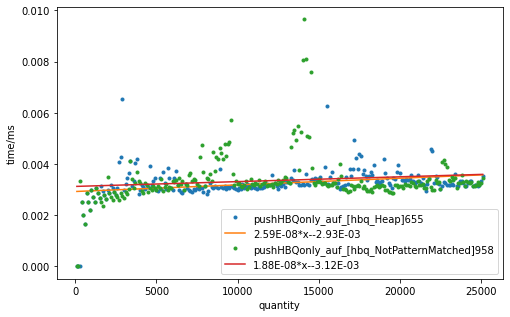
\includegraphics[scale=0.6]{Latex/Bilder/Plots/auf_heapOnly_pattern.png}
\caption{\label{fig:auf_hbqOnly_pattern} auf - vgl. Heap ohne Delivery Queue (mit und ohne PatternMatching)} 
\end{center}
\end{figure}

Zum Vergleich der beiden verschiedenen Implementierungen folgt ein Codeauszug aus der Holdback Queue ohne Pattern Matching. Dieses Beispiel soll die Tiefe des Codes und nicht die Funktionalität veranschaulichen, daher wird die Initialisierung mancher Parameter nicht gezeigt. 

\begin{lstlisting}
loop(HBQ, DLQ, Datei, Pos, DLQLimit) ->
	receive
		{From, {request, pushHBQ, [NNr, Msg, TSclientout]}} ->
			if 
				NNr < ExpNr ->
				true ->
					if
						Pos < (DLQLimit*2/3) ->
						true -> 
							if
								SNNr == ExpNr ->
								    ...
								true ->									
									...
					        end
			        end
	        end;
\end{lstlisting}

Nun folgt das Beispiel der Holdback Queue mit Pattern Matching. Auch hier wurden wieder große Teile des Codes entfernt, um nur die Tiefe zu verdeutlichen. Statt fast die gesamte Funktion in einem Block zu implementieren, werden hier die zwei Hilfsfunktionen pushHBQ/8 und pushHBQHelp/10 verwendet. \\


\begin{lstlisting}
loop(HBQ, DLQ, Datei, Pos, DLQLimit) ->
	receive
		{From, {request, pushHBQ, [NNr, Msg, TSclientout]}} ->
			pushHBQ([NNr, Msg, TSclientout, erlang:timestamp()], ExpNr, HBQ, DLQ, Datei, Pos, DLQLimit, From);
    ...
    
% --------------------------------------------------------------------------%
pushHBQ([NNr, _Msg, _TSclientout, _TShbqin], ExpNr, HBQ, DLQ, Datei, Pos, DLQLimit, From) when NNr < ExpNr -> ...;
pushHBQ([NNr, Msg, TSclientout, TShbqin], _ExpNr, HBQ, DLQ, Datei, Pos, DLQLimit, From) when Pos < (DLQLimit*2/3) -> ...;
pushHBQ([NNr, Msg, TSclientout, TShbqin], ExpNr, HBQ, DLQ, Datei, Pos, DLQLimit, From) ->
	pushHBQHelp([NNr, Msg, TSclientout, TShbqin], ExpNr, DLQ, Datei, Pos, DLQLimit, DLQMsg, SNNr, TempHBQ, From).

pushHBQHelp([NNr, Msg, TSclientout, TShbqin], ExpNr, DLQ, Datei, Pos, DLQLimit, DLQMsg, SNNr, TempHBQ, From) when SNNr == ExpNr -> ...;
pushHBQHelp([NNr, Msg, TSclientout, TShbqin], ExpNr, DLQ, Datei, Pos, DLQLimit, DLQMsg, SNNr, TempHBQ, From) -> ...;
\end{lstlisting}

Auffällig ist sofort, dass die erste Variante trotz der vielen Ebenen übersichtlicher wirkt als die zweite. Durch die vielen Parameter (pushHBQHelp/10 hat entsprechend zehn Parameter), welche den Hilfsfunktionen im unteren Auszug übergeben werden, strecken sich die Funktionsköpfe und sind schwer zu lesen. Letztendlich ist der Code aber kompakter und beim Hinzufügen weiterer Ebenen, wird wahrscheinlich die Variante mit dem Pattern Matching wieder übersichtlicher.\\
Die Zeitmessungen haben wie bereits erwähnt erwiesen, dass keine Variante effizienter als die andere ist. 
Laut dem von Erlang gegebenen 'Efficiency Guide' \footnote{\url{https://www.erlang.org/doc/efficiency_guide/functions.html#pattern-matching}} wird das Pattern Matching vom Kompiler zu einem switch-case generiert. 

\begin{lstlisting}
% Pattern Matching
foo(X, []) -> X;
foo(X, [Head|Tail]) -> Tail.
% wird zu Code kompiliert, welcher folgendem Beispiel gleicht:
foo(X,Y) ->
    case Y of
        [] -> X;
        [Head|Tail] -> Tail
    end.
\end{lstlisting}

Das switch-case Statement im Allgemeinen ist sehr effizient. Der Kompiler erstellt eine Art Tabelle mit den möglichen Werten, welche alle den gleichen Typen wie die übergebene Variable haben. Statt dann wie beim if-else Statement jede Bedingung zu prüfen, kann beim Aufruf des switch-case Statements der richtige Wert aus der Tabelle gesucht und der zugehörige Pfad ausgewählt werden. Ab fünf Fällen wird der switch-case deutlich effizienter als der if-else, da dann als Tabelle intern ein Lookup-Table oder eine Hash-List implementiert ist und somit alle Elemente innerhalb der gleichen Zeit gefunden werden können (frei nach \cite{geeksforgeeks}). Da in dem Code dieser Aufgabe nie mehr als fünf Fälle geprüft wurde, ist das Optimieren durch Pattern Matching hier nicht ausschlaggebend. Außerdem benötigen die Hilfsfunktionen und die vielen Parameter mehr Speicher und Zeit, diesen zu schreiben und zu lesen. Erkennen tut man dies an den Größen der Kompilierten beam-Dateien. Somit hat die kompilierte Datei der Holdback Queue ohne Pattern Matching 1kB (16\%) weniger als die andere. Im Plot der Abbildung \ref{fig:real_hbqAll} ist ab einer Eingabelistengröße von ca. 10000 auch zu erkennen, dass die Holdback Queue ohne Pattern Matching (die orange Trendlinie) leicht effizienter als die mit ist. \\
Beim Verwenden von wenig Parametern und wenig Hilfsfunktionen ist Pattern Matching also die bessere Variante, besonders, wenn mit vielen Fällen innerhalb der Funktion gearbeitet wird. 

\subsection{Alternative Anwendung}

Die Holdback und Delivery Queue in dieser Form können in vielen anderen Anwendungsgebieten angewendet werden. Dabei sollten aber Modifizierungen hinsichtlich der Sortieralgorithmen innerhalb der Holdback Queue vorgenommen werden. Wenn Werte aus einer großen Menge komplett zufällig an den Server gesendet werden und mehrere Clienten nun die Werte in richtiger Reihenfolge erwarten, dann sollte die Größe der Holdback Queue fast so groß, wie die der Wertemenge sein, damit keine Werte durch einen Overflow der Holdback Queue verloren gehen. Die interne Struktur der Holdback Queue wäre dann der Heap. Effizient wäre diese abstrakte Datenstruktur, da die Sortierung der Werte unabhängig von der Ausgabe an die Clients stattfindet. Würde nur die Holdback Queue genutzt werden und diese würde die Elemente über einen Heap sortieren, dann würde das kleinste Element als Wurzel solange dort stehen, bis alle Clients es empfangen haben und erst danach könnte das neue kleinste Element gesucht werden. 
Angenommen die Elemente werden in aufsteigender Reihefolge an den Server geschickt, wäre nur eine Delivery Queue am sinnvollsten, die Größe muss nicht der Wertemenge entsprechen, sondern hängt jetzt von der Geschwindigkeit der Clients ab.